\documentclass[a4paper,parskip,11pt, DIV12]{scrreprt}

\usepackage[english]{babel} % Für Deutsch [english] zu [ngerman] ändern. 
\usepackage[utf8]{inputenc}
\usepackage[T1]{fontenc}
%\usepackage{blindtext}
\usepackage{graphicx}
\usepackage{subfigure}
\renewcommand{\familydefault}{\sfdefault}
\usepackage{helvet}
\usepackage{fancyhdr}
\usepackage{amsmath}
\usepackage{mdwlist} %Benötigt für Abstände in Aufzählungen zu löschen
%\usepackage{here}
\usepackage{calc}
\usepackage{hhline}
\usepackage{marginnote}
\usepackage{chngcntr}
\usepackage{tabularx}
\usepackage{titlesec} % Textüberschriften anpassen

% \titleformat{Überschriftenklasse}[Absatzformatierung]{Textformatierung} {Nummerierung}{Abstand zwischen Nummerierung und Überschriftentext}{Code vor der Überschrift}[Code nach der Überschrift]

% \titlespacing{Überschriftenklasse}{Linker Einzug}{Platz oberhalb}{Platz unterhalb}[rechter Einzug]

\titleformat{\chapter}{\LARGE\bfseries}{\thechapter\quad}{0pt}{}
\titleformat{\section}{\Large\bfseries}{\thesection\quad}{0pt}{}
\titleformat{\subsection}{\large\bfseries}{\thesubsection\quad}{0pt}{}
\titleformat{\subsubsection}{\normalsize\bfseries}{\thesubsubsection\quad}{0pt}{}

\titlespacing{\chapter}{0pt}{-2em}{6pt}
\titlespacing{\section}{0pt}{6pt}{-0.2em}
\titlespacing{\subsection}{0pt}{5pt}{-0.4em}
\titlespacing{\subsubsection}{0pt}{-0.3em}{-1em}

%\usepackage[singlespacing]{setspace}
%\usepackage[onehalfspacing]{setspace}

\usepackage[
			%includemp,				%marginalien in Textkörper einbeziehen
			%includeall,
			%showframe,				%zeigt rahmen zum debuggen		
			marginparwidth=25mm, 	%breite der marginalien
			marginparsep=5mm,		%abstand marginalien - text
			reversemarginpar,		%marginalien links statt rechts
			%left=50mm,				%abstand von Seitenraendern
%			top=25mm,				%
%			bottom=50mm,
			]{geometry}		

%Bibliographie- Einstellungen
\usepackage[babel,german=quotes]{csquotes}
\usepackage[
   backend=bibtex8, 
   natbib=true,
    style=numeric,
    sorting=none
]{biblatex}
\bibliography{Quelle}
%Fertig Bibliographie- Einstellungen

\usepackage{hyperref}

\newenvironment{conditions}
  {\par\vspace{\abovedisplayskip}\noindent\begin{tabular}{>{$}l<{$} @{${}={}$} l}}
  {\end{tabular}\par\vspace{\belowdisplayskip}}

\begin{document}

\begin{titlepage}
\begin{figure}[h]
\hfill
\subfigure{\includegraphics[scale=0.04]{uzh}}
\end{figure}
\vspace{1 cm}
\textbf{\begin{huge}Data Analysis Project
\end{huge}}\\
\noindent\rule{\textwidth}{1.1 pt} \\

\begin{Large}\textbf{Designing a Particle Physics Experiment}
\end{Large}\\ 
\normalsize 
\par
\begingroup
\leftskip 0 cm
\rightskip\leftskip
\textbf{Module:}\\ PHY231 \\ \\
\textbf{Lecturer:}\\ Olaf Steinkamp \\ \\
\textbf{Assistants:}\\ Elena Graverini \& Andreas Weiden \\ \\
\textbf{Students:}\\ Nora Salgo, Manuel Sommerhalder, Tino Heuberger, Anar Bold \& Stefan Hochrein \\ \\
\textbf{Date of the assignment:}\\ 09.12.2016 \\ \\
\par
\endgroup
\clearpage



\end{titlepage}


%Start Layout
\pagestyle{fancy}
\fancyhead{} 
\fancyhead[R]{\small \leftmark}
\fancyhead[C]{\textbf{Designing a Particle Physics Experiment} } 
\fancyhead[L]{\includegraphics[height=2\baselineskip]{uzh}}

\fancyfoot{}
\fancyfoot[R]{\small \thepage}
\fancyfoot[L]{}
\fancyfoot[C]{}
\renewcommand{\footrulewidth}{0.4pt} 

\addtolength{\headheight}{2\baselineskip}
\addtolength{\headheight}{0.6pt}


\renewcommand{\headrulewidth}{0.6pt}
\renewcommand{\footrulewidth}{0.4pt}
\fancypagestyle{plain}{				% plain redefinieren, damit wirklich alle seiten im gleichen stil sind (ausser titlepage)
\pagestyle{fancy}}

\renewcommand{\chaptermark}[1]{ \markboth{#1}{} } %Das aktuelle Kapitel soll nicht Gross geschriben und Nummeriertwerden

\counterwithout{figure}{chapter}
\counterwithout{table}{chapter}
%Ende Layout

%\tableofcontents

\chapter{Introduction}

This is the report for the K2Pi assignment for the data analysis project. In this report we will document our results and how we derived them.

\subsection*{The experiment}

The experiment, which is called K2Pi, analyses the decay of positively charged kaons $K^+$ into one positively charged and one neutral pion ($\pi^+$ and a $\pi^0$), where the lifetime of a $K^+$ can be determined by analysing the data from an earlier experiment called LifeK.

\begin{figure}[h] 
\centering
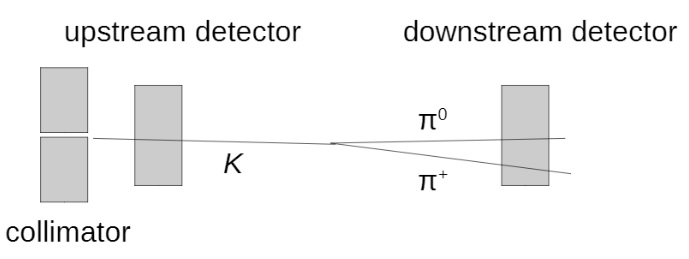
\includegraphics[width=0.75\textwidth]{ExperimentSetup.jpg} 
\caption{Experimental setup}
\label{fig:1}    
\end{figure}

As we can see, we have a collimator which generates a beam of $K^+$ particles. Furthermore, we have two detectors placed at a certain distance from each other along the flight path of the $K^+$. The first detector is called the "Upstream detector" and measures the direction and the momentum of the kaons in the beam. The second detector, called "Downstream detector", is composed of a tracking detector to detect the $\pi^+$ and a calorimeter to measure the $\pi^0$.
\\
\\
However, the pions also have an average lifetime which is given by $\tau_{\pi^+} = 2.6 \cdot 10^{-8}s$. This results in an average decay length of $\beta \gamma c\tau_{\pi^+} = 4.188$km.

For the purpose of the project we've been told to assume that the $\pi^+$ is stable and does not decay during the process. We now have to create a simulation to simulate this decay and find the optimum distance between the two detectors in order to capture as many events as possible, where a successful event is considered the detection of both pions corresponding to the same kaon decay. In the first part of the simulation, we will assume a stream that has no spread and moves exactly on the z-axis. For the second part we will add a spread to the stream coming from the collimator following a Gaussian distribution.

\clearpage

\chapter{Lifetime}

\clearpage


\chapter{Experimental Strategy}


We split the $K^+$ decay process and its detection in several distinct parts.

\section{Simulation of the Kaon Decay} \label{sec:kdecay}

At first, we defined a function that returns the position vector $P_{decay}$ of one single kaon decay in Cartesian coordinates and its two deflection angles with respect to the z-axis. These angles ($\alpha$ in x-direction and $\beta$ in y-direction) are random variables following a Gaussian distribution with $\mu$ = 0 and $\sigma_x$ = $\sigma_y$ = 1 mrad. The modulus is also a random variable but follows an exponential distribution with $\tau$ = $\tau_{K^+}$, which was derived in the first part of the assignment.

For the actual $K^+$ decay into pions, we defined a function that simulates the decay in the $K^+$ rest frame and boosts the momentum 4-vectors to the lab frame.
 First, it creates the direction vector of the $\pi^0$-momentum in the $K^+$ rest frame in standard spherical coordinates where the angle $\theta$ is a random variable, uniformly distributed in a range from 0 to $\pi$ and $\varphi$ is uniformly distributed in a range from 0 to 2$\pi$. 
\begin{figure}[h] 
\centering
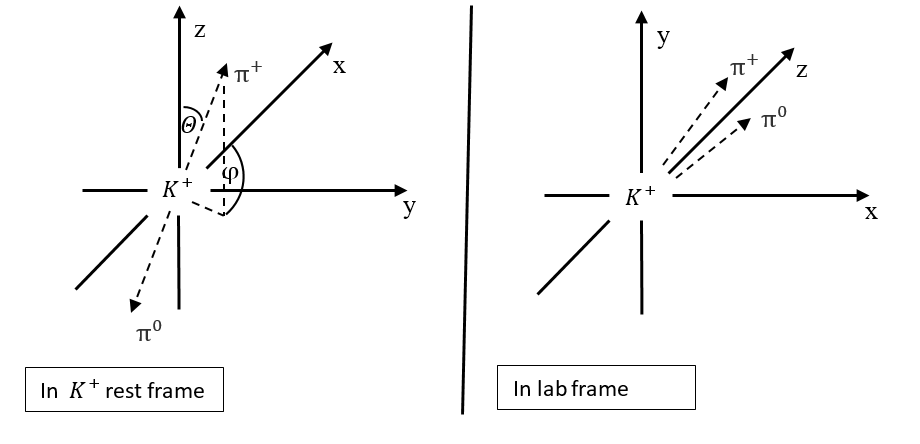
\includegraphics[width=0.75\textwidth]{Frames.png} 
\caption{$K^+$ into $\pi^0$ and $\pi^+$ in rest frame and in lab frame}
\label{fig:2}    
\end{figure}
From this follows the momentum vector $p^*_{\pi^0}$ of the $\pi^0$ by translating to Cartesian coordinates and multiplying the expected modulus $|p^*_{\pi}|$ of the $\pi$ momentum computed in section \ref{sec:gammabeta}. The corresponding $\pi^+$ momentum vector $p^*_{\pi^+}$ is derived by changing the sign since the pions are assumed to be produced isotropically with back-to-back momentum and from momentum conservation follows that their modulus needs to be equal. 
\begin{equation}
p^*_{\pi^0} = |p^*_{\pi}| \cdot \begin{bmatrix}
\sin\theta \cdot \cos\varphi \\ \sin\theta \cdot \sin\varphi \\ \cos\theta
\end{bmatrix}
, \quad \quad p^*_{\pi^+} = -p^*_{\pi^0}
\end{equation}
The corresponding energy values $E^*_{\pi}$, also computed in section \ref{sec:gammabeta}, are amended in order to represent the data as momentum 4-vectors $P^*_{\pi}$  prevalent in special relativity. These vectors are then boosted to the lab frame by multiplying them with the matrix representation of Lorentz boost in the z'-direction whose $\beta$- and $\gamma$-factors are computed in section \ref{sec:pE}.
\begin{equation}
P_{\pi} = 
\begin{bmatrix}
E_{\pi} \\ p_{\pi,x'} \\ p_{\pi,y'} \\ p_{\pi,z'}
\end{bmatrix}
=
\begin{bmatrix}
\gamma & 0 & 0 & \beta \gamma \\
0 & 1 & 0 & 0 \\
  0 & 0 & 1 & 0\\
  \beta \gamma & 0 & 0 & \gamma \\
\end{bmatrix}
\cdot
\begin{bmatrix}
E_{\pi}^* \\ p_{\pi,x'}^* \\ p_{\pi,y'}^* \\ p_{\pi,z'}^*
\end{bmatrix} = P^*_{\pi}
\end{equation}
The z'-axis here corresponds to the direction of the $K^+$-velocity which is only equivalent to the z-axis of the lab frame in case of an idealized non deflected $K^+$-beam. The three momentum components in the x'-, y'-, and z'-direction of the resulting 4-vectors in the lab frame are thus rotated by the angles $\alpha$ around the y-axis and $\beta$ around the x-axis by multiplying them by the corresponding rotation matrices:
\begin{equation}
\begin{bmatrix}
p_{\pi,x} \\ p_{\pi,y} \\ p_{\pi,z}
\end{bmatrix}
=
\begin{bmatrix}
1 &   0         & 0           \\
0 & \cos \beta & -\sin \beta \\
0 & \sin \beta &  \cos \beta
\end{bmatrix}
\cdot
\begin{bmatrix}
\cos \alpha  & 0 & \sin \alpha \\
   0         & 1 &  0          \\
-\sin \alpha & 0 & \cos \alpha
\end{bmatrix}
\cdot
\begin{bmatrix}
p_{\pi,x'} \\ p_{\pi,y'} \\ p_{\pi,z'}
\end{bmatrix}
\end{equation}

\clearpage


\section{Pion Detection} \label{sec:pdetection}

Knowing the point $P_{decay}=(x_K,y_K,z_K)$  where the kaon decays and the directions $\vec{e}_{\pi^+}=(x_{\pi^+},y_{\pi^+},z_{\pi^+})$ and $\vec{e}_{\pi^0}=(x_{\pi^0},y_{\pi^0},z_{\pi^0})$ in which the pions fly after the decay (derived from the momentum vectors $p_{\pi}$), we can now determine if both $\pi$ are detected by performing a linear combination. The condition is that the z components of the points $P_{detect,\pi^+}$,$P_{detect,\pi^0}$, where the pions are detected, are equal to the z components of the position of our detector, which we call $a$. This leads to the following equations:
\begin{align*}
a &= z_K + n_{\pi^+} \cdot z_{\pi^+} \\ 
a &= z_K + n_{\pi^0} \cdot z_{\pi^0}
\end{align*} 
Solving for $n_{\pi^+}$ and  $n_{\pi^0}$ leads to: 
\begin{align*}
n_{\pi^+} &= (a-z_1)/z_{\pi^+}\\
n_{\pi^0} &= (a-z_1)/z_{\pi^0}
\end{align*}
With these $n_{\pi^+}$ and $n_{\pi^0}$ the x and y coordinates of $P_{detect,\pi^+}$ and $P_{detect,\pi^0}$ can be calculated by:
\begin{align*}
x_{\pi^+} &= x_K+n_{\pi^+} \cdot x_{\pi^+}\\
y_{\pi^+} &= y_K+n_{\pi^+} \cdot y_{\pi^+}\\
x_{\pi^0} &= x_K+n_{\pi^0} \cdot x_{\pi^0}\\
y_{\pi^0} &= y_K+n_{\pi^0} \cdot y_{\pi^0}\\
\end{align*}
Now the distance to the center of the detector of $P_{detect,\pi^+}$ and $P_{detect,\pi^0}$ can easily be calculated by:
\begin{align*}
d_{\pi^+} &= \sqrt{x_{\pi^+}^2 + y_{\pi^+}^2}\\
d_{\pi^0} &= \sqrt{x_{\pi^0}^2 +  y_{\pi^0}^2} 
\end{align*}
Because the detector is radially symmetric around the z-axis with radius $r=2m$, every decay with $d_{\pi^+} \leq r$ and $d_{\pi^0} \leq r$ can be rated as a success. Every decay with at least one of the corresponding pions not detected is rated as a failure. 
If the z component of the kaon decay point is greater than $a$ and thus the $K^+$ decays after the detector, the event is obviously also rated as a failure. 

\clearpage


\section{Run Experiment}

Now being able to rate one event as success or failure, the experiment can be performed. In order to save computing time and also to ensure maximum comparability, a list of decay points is generated first with corresponding lists of the directions of the $\pi^+$ and the $\pi^0$ as described in section \ref{sec:kdecay}. 
Then for every decay point with $\pi^0$ and $\pi^+$ directions, success or failure is determined as described in section \ref{sec:pdetection}. With this information a success rate for the lists can be calculated for a certain distance a (z component of the position of the detector). The success rate was simply calculated by the number of successes divided by the total number of trials. By varying the distance a, and calculating the success rate for each of its values the optimal position was determined.

\clearpage


\chapter{Conclusion}

The higher the number of iterations for the $\tau$ estimation and the $K^+$ decay simulation, the more accurate the results become. 
Also, the difference between the simulation with and without the spread at the collimator is quite noticeable. The success rate gets smaller when spreading is enabled and the whole graph gets “shifted” to the right, increasing the optimal distance between the two sensors. 
With the multithreaded enabled python script “K2pi.py”, we could simulate the decay for large $n$ quite easily. This is the result for $n = 100’000$ with a spread of $\sigma_x=\sigma_y=1$ mrad:

\begin{figure}[h] 
\centering
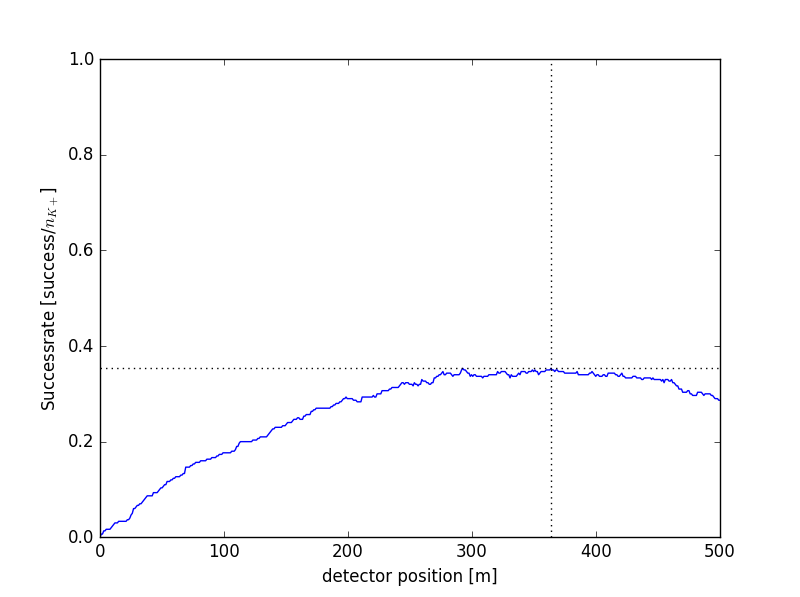
\includegraphics[width=0.7\textwidth]{Simulation50.png} 
\caption{Result}
\label{fig:Zee}    
\end{figure}

Where the optimal distance is at $295.8m$ with a maximum efficiency of $32.6 \%$. As we can see the cruve is very flat at its peak and therefore the distance between the two sensors does not have to be very precise. Looking at the graph somewhere at $300m \pm 50m$ should be fine and yields only very small differences in the efficiency of the experiment. 
With spread $= 0$ and $n = 100000$ we get the following result:

\clearpage

\chapter{Physical Calculations}

\section{Kaon relativistic $\gamma$- and $\beta$-factor} \label{sec:gammabeta}

We know the momentum of the $K^+$: $p_{K^+} = 75 GeV/c$\\
From this we can find the velocity of the $K^+$ by the formula:
\begin{equation}
p_{K^+} = \gamma \cdot m_{0K^+} \cdot v
\end{equation}
$\Rightarrow$
$v/c = \beta = 0.99997834$ ;
$\gamma = 151.92448660$\\

\section{Pion Momentum and Energy} \label{sec:pE}

The decay products are produced isotropically, so the momenta of the decay products are equal in modulus and are in opposite direction. 
So in the $K^+$ rest frame the momenta are conserved:
\begin{equation}
\overrightarrow{p}_{K^+} = \overrightarrow{p}_{\pi^0} + \overrightarrow{p}_{\pi^+} = 0
\end{equation}

In modulus:
\begin{equation}
p_{\pi^0} = p_{\pi^+} = p
\end{equation}

The decay obey the law of energy conservation in the $K^+$ rest frame:
\begin{equation}
E_{K^+} = E_{\pi^0} + E_{\pi^+}
\end{equation}

$\Rightarrow$
\begin{equation}
m_{0K^+}c^2 = \sqrt{p^2c^2 + m_{0\pi^0}^2c^4} + \sqrt{p^2c^2 + m_{0\pi^+}^2c^4}
\end{equation}

The rest masses:
\begin{eqnarray}
m_{0\pi^0} = 134.9766 MeV/c^2\\
m_{0\pi^+} = 139.5702 MeV/c^2\\
m_{0K^+} = 493.677 MeV/c^2
\end{eqnarray}

For the momentum of the pions we get:\\

\begin{equation}
p = 205.138 MeV/c
\end{equation}

The total energy of the pions are calculated by the following formula:
\begin{eqnarray}
E_{\pi^0} = \sqrt{p^2c^2 + m_{0\pi^0}^2c^4} = 245.5611565 MeV\\
E_{\pi^+} = \sqrt{p^2c^2 + m_{0\pi^+}^2c^4}= 248.115779 MeV
\end{eqnarray}


\clearpage  

%\renewcommand{\bibname}{Quellenverzeichnis}
%\printbibliography

\end{document}
